\documentclass{article}

\usepackage{geometry}
\usepackage{amsmath}
\usepackage{graphicx, eso-pic}
\usepackage{listings}
\usepackage{hyperref}
\usepackage{multicol}
\usepackage{fancyhdr}
\usepackage{tikz}
\pagestyle{fancy}
\fancyhf{}
\hypersetup{ colorlinks=true, linkcolor=black, filecolor=magenta, urlcolor=cyan}
\geometry{ a4paper, total={170mm,257mm}, top=40mm, right=20mm, bottom=20mm, left=20mm}
\setlength{\parindent}{0pt}
\setlength{\parskip}{0.5em}
\renewcommand{\headrulewidth}{0pt}
\AddToShipoutPictureBG{%
  \AtPageUpperLeft{%
    \raisebox{-\height}{
\includegraphics[width=\paperwidth, height=30mm]{headerarkav.png}}
  }
}
\rfoot{\thepage}
\lfoot{Competitive Programming - Arkavidia 8.0}
\lstset{
    basicstyle=\ttfamily\small,
    columns=fixed,
    extendedchars=true,
    breaklines=true,
    tabsize=2,
    prebreak=\raisebox{0ex}[0ex][0ex]{\ensuremath{\hookleftarrow}},
    frame=none,
    showtabs=false,
    showspaces=false,
    showstringspaces=false,
    prebreak={},
    keywordstyle=\color[rgb]{0.627,0.126,0.941},
    commentstyle=\color[rgb]{0.133,0.545,0.133},
    stringstyle=\color[rgb]{01,0,0},
    captionpos=t,
    escapeinside={(\%}{\%)}
}

\begin{document}

\begin{center}
    \section*{D. Demi Keabadian} % ganti judul soal

    \begin{tabular}{ | c c | }
        \hline
        Batas Waktu  & 2s \\    % jangan lupa ganti time limit
        Batas Memori & 512MB \\  % jangan lupa ganti memory limit
        \hline
    \end{tabular}
\end{center}

\subsection*{Deskripsi}
Diketahui terdapat sebuah pohon suci berakar yang terdiri atas $M$ buah simpul. Setiap simpul dinomori dari $1$ hingga $M$ dengan akar pohon berada pada simpul $1$. Simpul $i$ dari pohon tersebut memiliki nilai kesucian $X_i$ dan nilai keindahan $W_i$. Tidak ada dua simpul yang memiliki nilai keindahan yang sama.

Definisikan sebuah \textbf{array bagus} adalah sebuah \textit{array} $A$ (awalnya kosong) yang dibangun dengan melakukan operasi berikut sebanyak $N$ kali.

\begin{enumerate}
    \item Pilih sebuah simpul $i$.
    \item Tambahkan $W_i$ menjadi elemen terakhir $A$.
\end{enumerate}

Definisikan \textbf{keajaiban-$S$} dari sebuah simpul $i$ adalah frekuensi kemunculan $W_i$ pada sebuah \textbf{array bagus} $S$.

Simpul $u$ dapat \textbf{memberkati array bagus} $S$ jika jumlah \textbf{keajaiban-$S$} dari semua simpul yang merupakan elemen subpohon simpul $u$ tidak melebihi $X_u$,  nilai kesucian simpul $u$.

Sebuah \textit{array} dikatakan \textbf{sempurna} jika \textit{array} tersebut merupakan \textbf{array bagus} dan semua simpul dari pohon suci \textbf{memberkati} \textbf{array} tersebut.

\textit{Array} yang \textbf{sempurna} memiliki nilai kesempurnaan yang merupakan perkalian semua elemen yang berada pada \textit{array} tersebut.

Diketahui bahwa pohon suci ini memiliki sebuah legenda. "Barangsiapa yang mampu mencari jumlah semua nilai kesempurnaan dari setiap \textbf{array sempurna} berbeda yang mungkin, dia akan diberikan imbalan berupa keabadian".

Arka merupakan seorang \textit{wizard} yang sudah meneliti pohon suci ini bertahun-tahun. Namun Arka menyadari satu hal dan mencoba untuk bernegosiasi dengan pohon suci. "Wahai yang mulia pohon, kesempurnaan semua \textit{array} yang sempurna bisa memberikan nilai yang tak terjangkau, mohon dipertimbangkan kembali".

Karena kemuliaannya, pohon suci tersebut akhirnya mendengar keluhan sang \textit{wizard} dan hanya memerlukan hasil yang telah dimodulo dengan $998244353$. Sayangnya Arka masih kesulitan untuk mendapatkan hasil yang diinginkan dan meminta bantuan Anda untuk membantu Arka mencapai keabadian.


\subsection*{Format Masukan}
Baris pertama terdiri dari dua bilangan bulat $N$ dan $M$ ($1 \leq N \leq 3 \times 10^4, 1 \leq M \leq 100$) yang masing-masing menyatakan panjang \textit{array bagus} dan jumlah simpul pada pohon suci.

Baris berikutnya berisi $M$ nilai kesucian $X_{i}$ $(0 \leq X_{i} \leq 3 \times 10^4)$. 

Baris berikutnya berisi $M$ nilai keindahan $W_i$ $(1 \leq W_{i} \leq 10^9)$.

$M - 1$ baris berikutnya berisi dua bilangan bulat $U$ dan $V$ ($1 \leq U, V \leq M$) yang menyatakan terdapat sisi yang menghubungkan simpul $U$ dan simpul $V$.


\subsection*{Format Keluaran}
Keluarkan bilangan bulat yang menyatakan hasil jumlah nilai kesempurnaan semua \textit{array sempurna} berbeda yang mungkin dibangun dimodulo dengan $998244353$.

\pagebreak

\begin{multicols}{2}
\subsection*{Contoh Masukan 1}
\begin{lstlisting}
4 6
4 0 3 4 2 4
2 4 8 16 32 64
1 2
2 3
3 4
2 5
5 6

\end{lstlisting}
\columnbreak
\subsection*{Contoh Keluaran 1}
\begin{lstlisting}
16
\end{lstlisting}
\end{multicols}

\begin{multicols}{2}
\subsection*{Contoh Masukan 2}
\begin{lstlisting}
8 8
8 5 7 7 3 8 2 1
2 10 11 3 6 19 22 42
1 2
1 3
2 4
2 5
5 6
5 7
5 8

\end{lstlisting}
\columnbreak
\subsection*{Contoh Keluaran 2}
\begin{lstlisting}
588486564
\end{lstlisting}
\end{multicols}

\subsection*{Penjelasan}
Pada contoh masukan pertama, pohon suci dapat digambarkan sebagai berikut.
\begin{center}
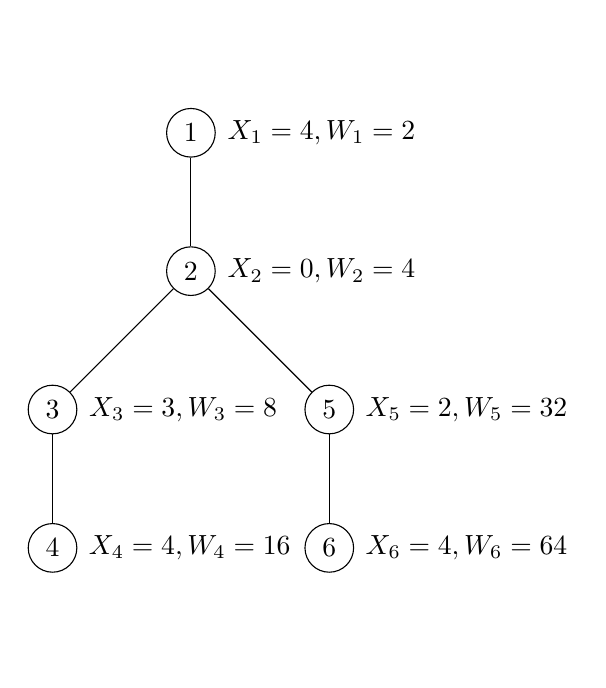
\begin{tikzpicture}
[sibling distance=10em,level distance=5em,
every node/.style={shape=circle,draw,align=center}]
\node [label=360:{$X_1 = 4, W_1 = 2$}]{1}
    child{node [label=360:{$X_2 = 0, W_2 = 4$}]{2}
        child{node [label=360:{$X_3 = 3, W_3 = 8$}]{3}
            child{node [label=360:{$X_4 = 4, W_4 = 16$}]{4}}}
        child{node [label=360:{$X_5 = 2, W_5 = 32$}]{5}
            child{node [label=360:{$X_6 = 4, W_6 = 64$}]{6}}}};
\end{tikzpicture}
\end{center}

Karena $X_{2}$ bernilai 0, elemen dari simpul yang merupakan bagian dari subpohon simpul 2 tidak dapat diambil sama sekali. Oleh karena itu, satu-satunya kemungkinan \textit{array sempurna} yang dapat dibentuk adalah [2, 2, 2, 2] yang nilai kesempurnaannya adalah 16, sehingga keluaran dari contoh ini bernilai 16.

\pagebreak

\end{document}